\newthought{\textbf{Nurani Harum Fardaniah - 2020903430034 - TRKJ 3B}}

\newday{\textbf{1 - 2 Desember 2022} - Instalasi dan Konfigurasi Apache Hadoop}
\begin{enumerate}
\item Kendala dan Solusi \\
Kendala :\\
Saat melakukan penginstalan hadoop tidak ada kendala apapun. Namun pada saat melakukan konfigurasi hadoop terdapat kendala pada saat melakukan hdfs namenode -format. Perintah ini tidak mau dijalankan karena ada kesalahan dalam penulisan pada file core-site.xml
Saat melakukan perintah jps pun hanya menampilkan 1 saja.

Solusi :\\
Melakukan perubahan penulisan pada file core-site.xml, setelah itu perintah hdfs namenode -format dapat dijalankan dan saat melakukan perintah jps akhirnya muncul ada 5.

\item Kesimpulan \\
Praktikum penginstalan hadoop dan konfigurasi hadoop berhasil dijalankan sesuai perintah-perintah yang ada.

\begin{figure}[!ht]
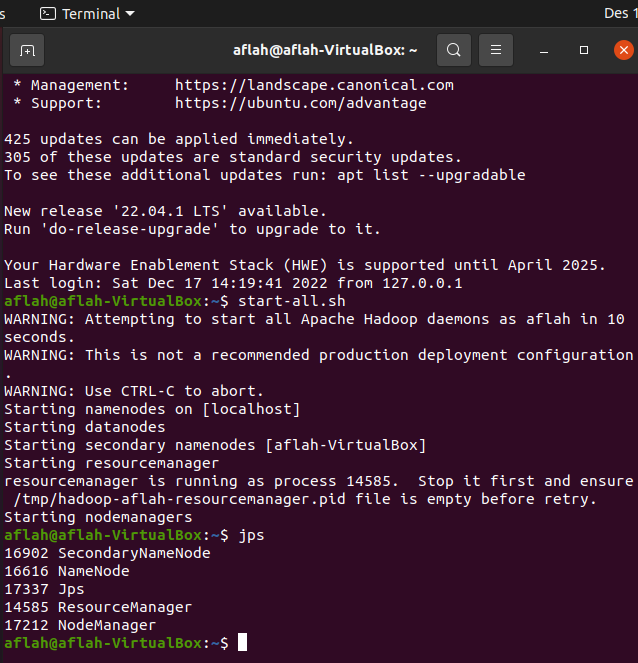
\includegraphics[width=\textwidth]{NuraniHarumFardaniah/jps}
\caption{hasil dari jps}
\label{gam:perkuliahan-25-11}
\end{figure}

\begin{figure}[!ht]
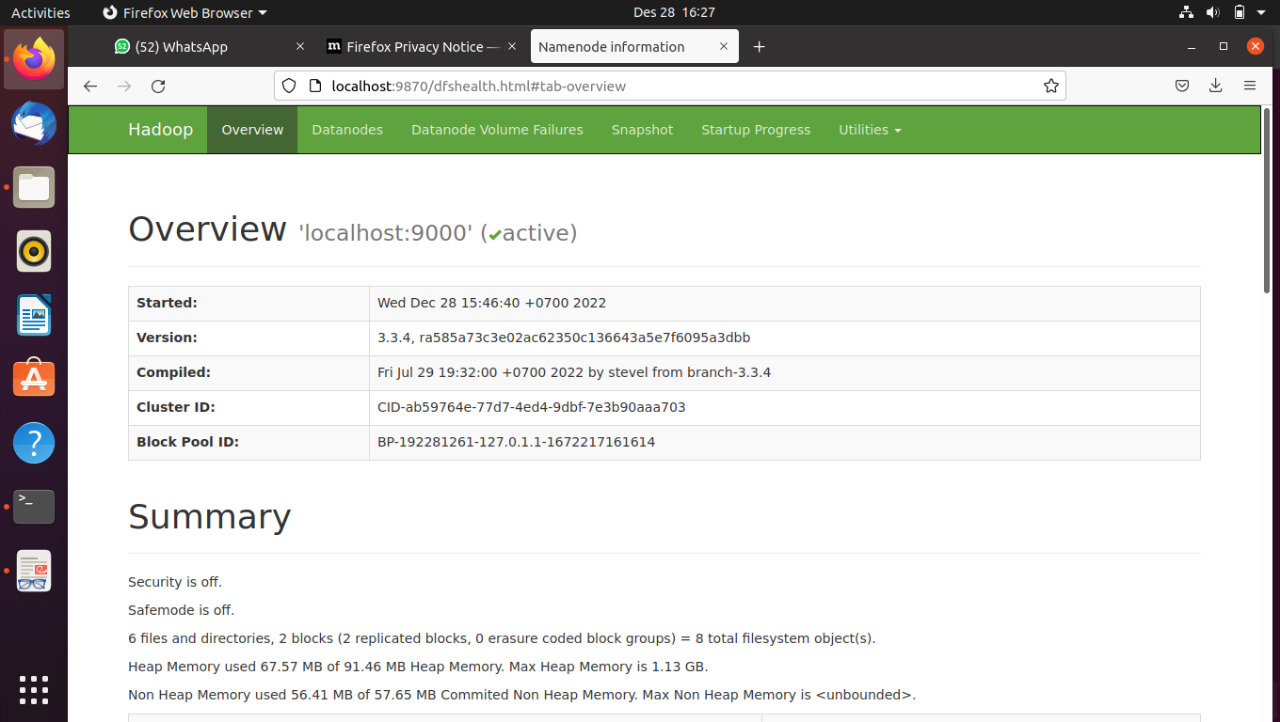
\includegraphics[width=\textwidth]{NuraniHarumFardaniah/localhost9870}
\caption{hasil dari localhost 9870}
\label{gam:perkuliahan-25-11}
\end{figure}

\newpage
\begin{figure}[!ht]
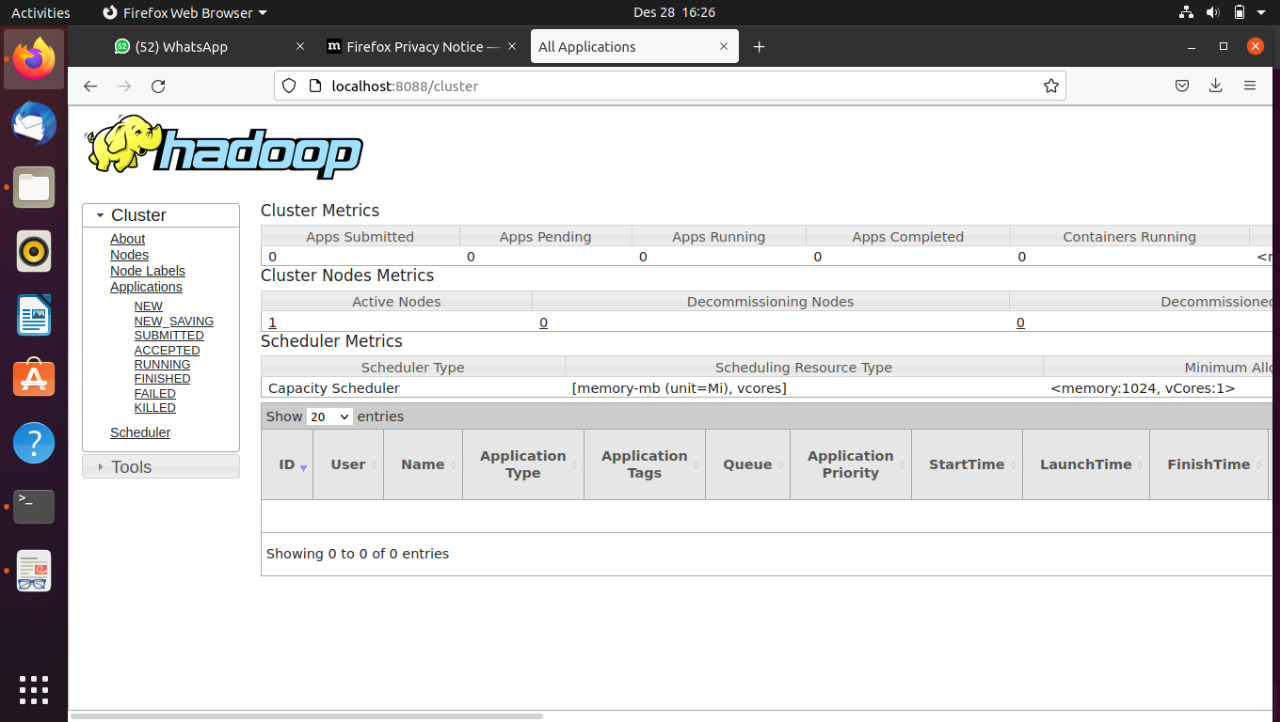
\includegraphics[width=\textwidth]{NuraniHarumFardaniah/localhost8088}
\caption{hasil dari localhost 8088}
\label{gam:perkuliahan-25-11}
\end{figure}

\end{enumerate}

\newday{\textbf{8 Desember 2022}} 
\begin{enumerate}
\item Kendala dan Solusi

\item Kesimpulan

\end{enumerate}

\newday{\textbf{9 Desember 2022}} 
\begin{enumerate}
\item Kendala dan Solusi

\item Kesimpulan

\end{enumerate}

\newday{\textbf{15 Desember 2022} - WordCount Bawaan Java}
\begin{enumerate}
\item Kendala dan Solusi
\newline Tidak ada kendala apapun saat melakukan program WordCount bawaan Hadoop

\item Kesimpulan
\newline Praktikum berhasil dilakukan sesuai dengan perintah-perintah yang ada. WordCount sendiri merupakan program untuk menghitung jumlah kata yang ada pada data.


\begin{figure}[!ht]
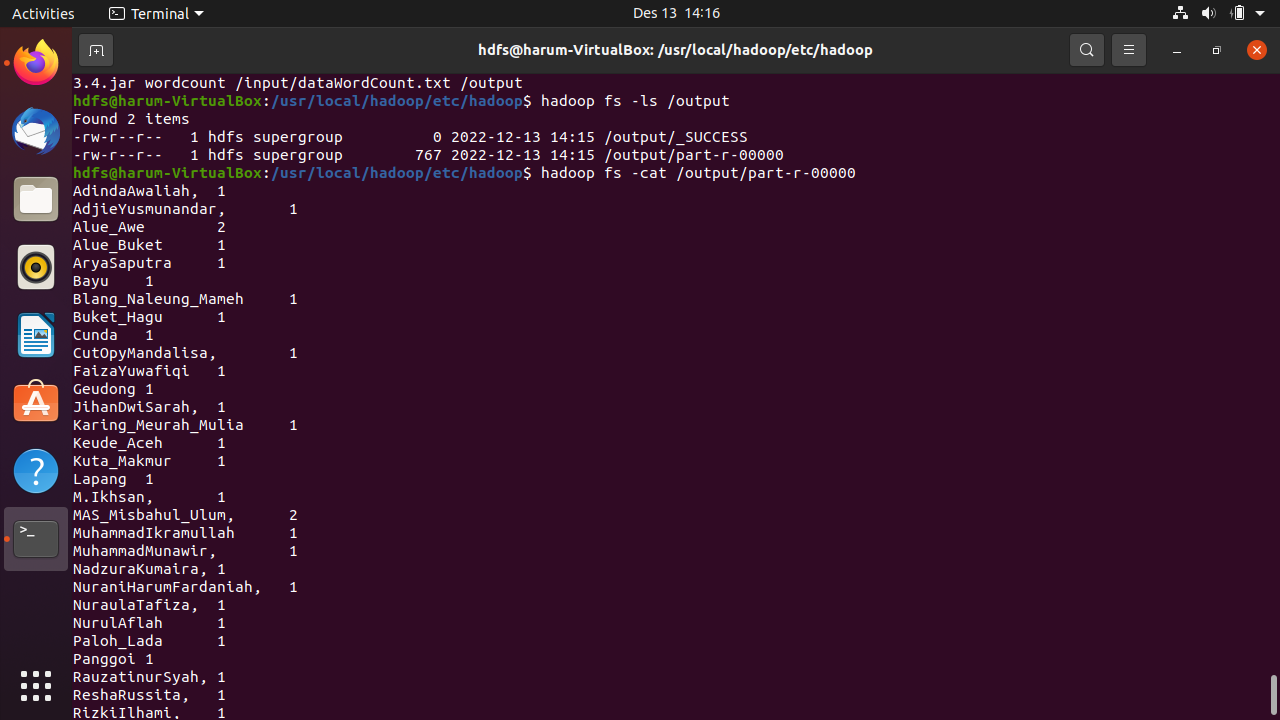
\includegraphics[width=\textwidth]{NuraniHarumFardaniah/6-7a}
\caption{Hasil dari langkah 6 dan 7}
\label{gam:perkuliahan-25-11}
\end{figure}
\newpage
\begin{figure}[!ht]
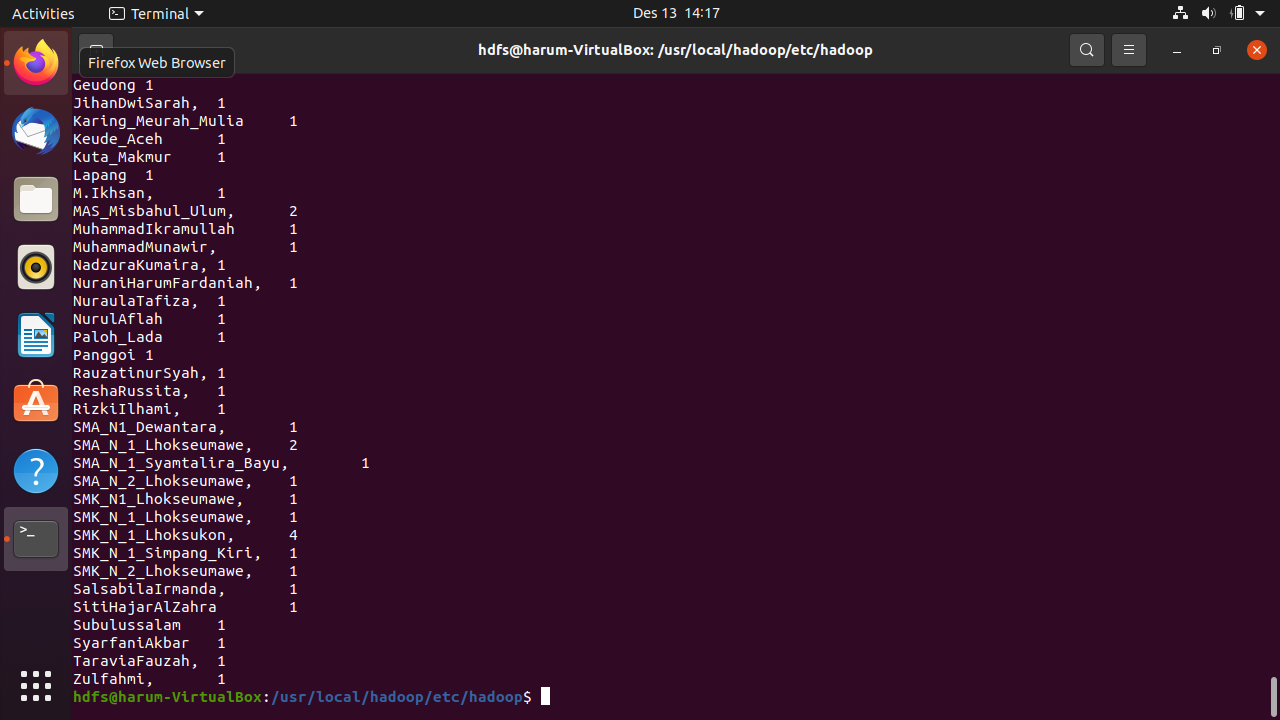
\includegraphics[width=\textwidth]{NuraniHarumFardaniah/7b}
\caption{Hasil dari langkah 7}
\label{gam:perkuliahan-25-11}
\end{figure}

\end{enumerate}

\newday{\textbf{16 Desember 2022} - WordCount dengan Java}
\begin{enumerate}
\item Kendala dan Solusi
\newline Kendala :\\
Saat melakukan praktikum program WordCount dengan Java terdapat kendala pada saat melakukan compile file WordCount. Perintah ini tidak mau dijalankan karena ada kesalahan dalam penulisan pada file WordCount.java

Solusi :\\
Melakukan perubahan penulisan pada file WordCount.java, setelah itu perintah untuk melakukan compile pada file WordCount.java dapat dijalankan.

\item Kesimpulan
\newline Praktikum berhasil dilakukan sesuai dengan perintah-perintah yang ada. Data pada WordCount dapat ditampilkan sesuai dengan yang telah dibuat.


\begin{figure}[!ht]
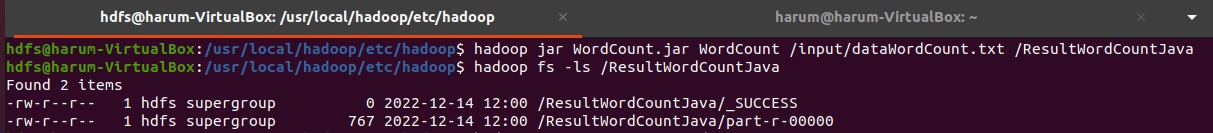
\includegraphics[width=\textwidth]{NuraniHarumFardaniah/9}
\caption{Hasil Perhitungan dengan WordCount Hadoop}
\label{gam:perkuliahan-25-11}
\end{figure}

\begin{figure}[!ht]
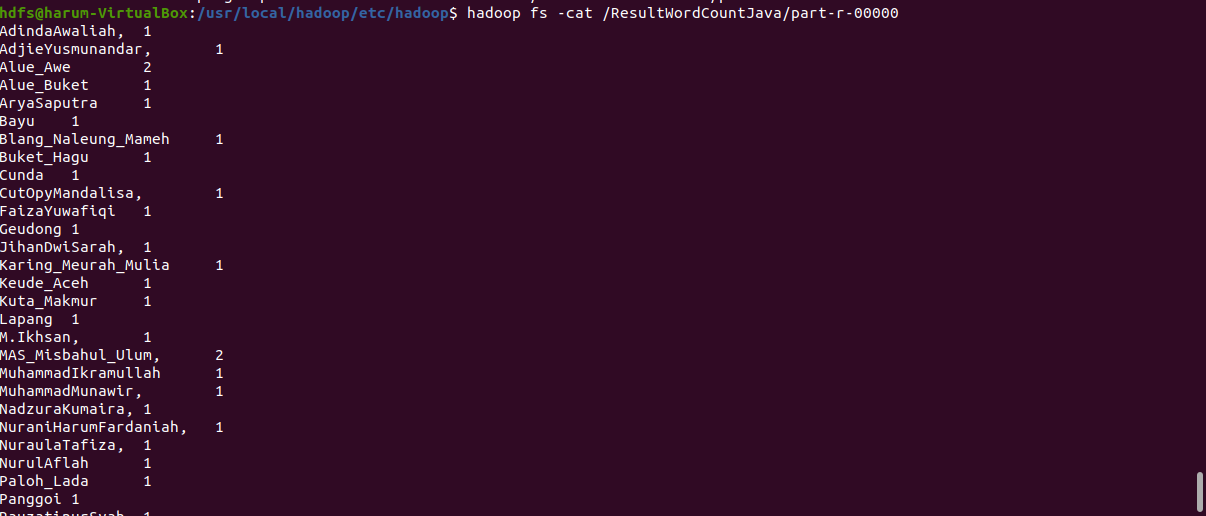
\includegraphics[width=\textwidth]{NuraniHarumFardaniah/10a}
\caption{Hasil Perhitungan dengan WordCount Hadoop}
\label{gam:perkuliahan-25-11}
\end{figure}
\newpage
\begin{figure}[!ht]
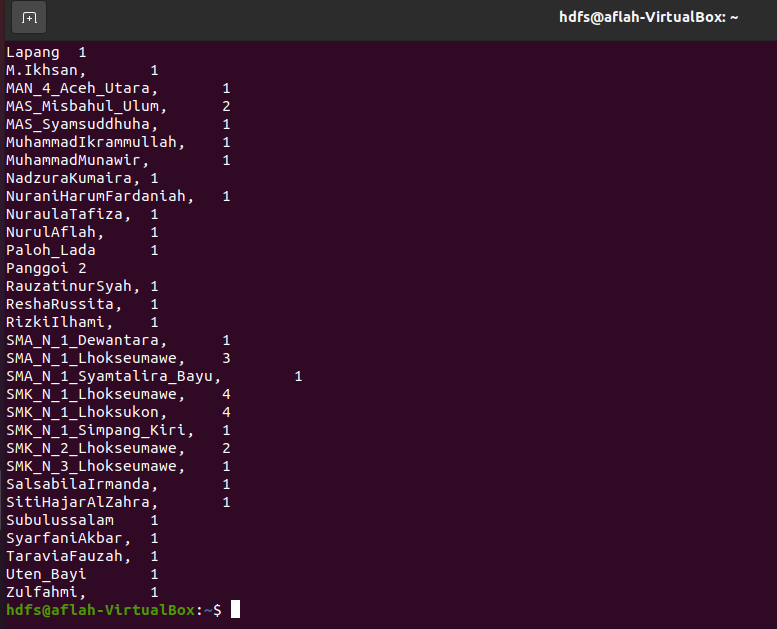
\includegraphics[width=\textwidth]{NuraniHarumFardaniah/10b}
\caption{Hasil Perhitungan dengan WordCount Hadoop}
\label{gam:perkuliahan-25-11}
\end{figure}

\end{enumerate}

\newday{\textbf{22 Desember 2022}- Instalasi Apache Spark (PySpark)} 
\begin{enumerate}
\item Kendala dan Solusi
\newline Pada saat penginstalan Apache Spark (PySpark) tidak ada kendala apapun

\item Kesimpulan
\newline Proses penginstalan Apache Spark berhasil dilakukan tanpa adanya kendala satupun
\newpage
\begin{figure}[!ht]
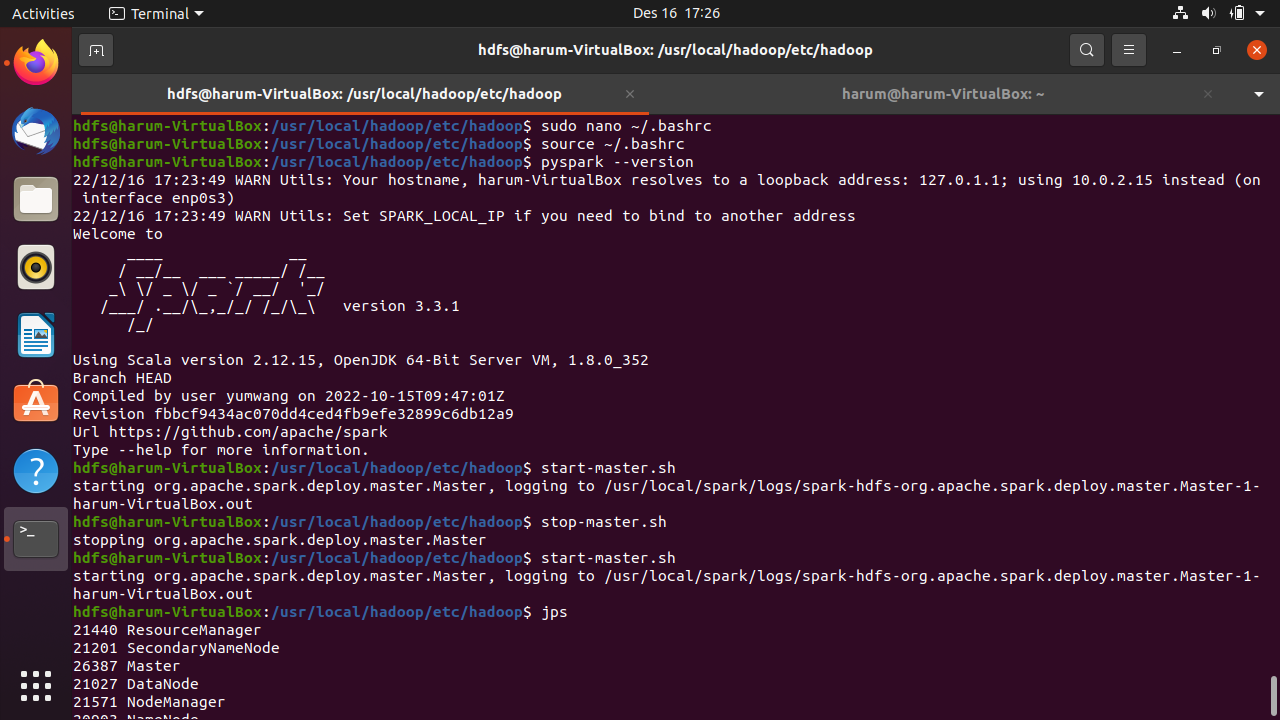
\includegraphics[width=\textwidth]{NuraniHarumFardaniah/sparkversion}
\caption{Hasil Instalasi Spark}
\label{gam:perkuliahan-25-11}
\end{figure}

\end{enumerate}

\newday{\textbf{23 Desember 2022}- Program WordCount dengan Python} 
\begin{enumerate}
\item Kendala dan Solusi
\newline Terdapat kendala tidak bisa menjalankan program hadoop
python. Terdapat pesan error 'Streaming Command Failed' seperti gambar di bawah ini :

\begin{figure}[!ht]
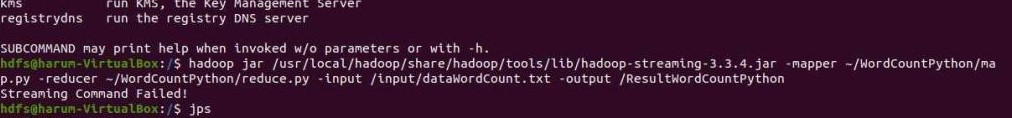
\includegraphics[width=\textwidth]{NuraniHarumFardaniah/kendala}
\caption{Kendala menjalankan Hadoop Python}
\label{gam:perkuliahan-25-11}
\end{figure}

\item Kesimpulan
\newline Belum ada hasil akhir, karena masih ada kendala. Masih mencoba sampai berhasil
\end{enumerate}

\newday{\textbf{25 Desember 2022}- Program WordCount dengan PySpark} 
\begin{enumerate}
\item Kendala dan Solusi
\newline Saat menjalankan program WordCount dengan menggunakan PySpark, tidak ada kendala apapun
\item Kesimpulan
\newline Program WordCount dengan menggunakan PySpark berhasil dilakukan

\newpage
\begin{figure}[!ht]
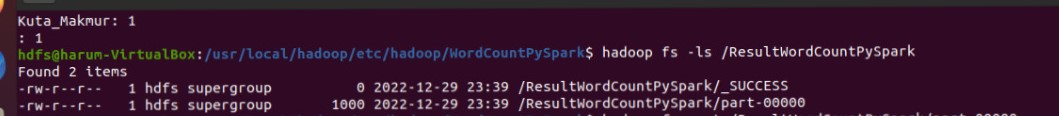
\includegraphics[width=\textwidth]{NuraniHarumFardaniah/pyspark6}
\caption{Cek hasil ResultWordCountPyspark}
\label{gam:perkuliahan-25-11}
\end{figure}

\begin{figure}[!ht]
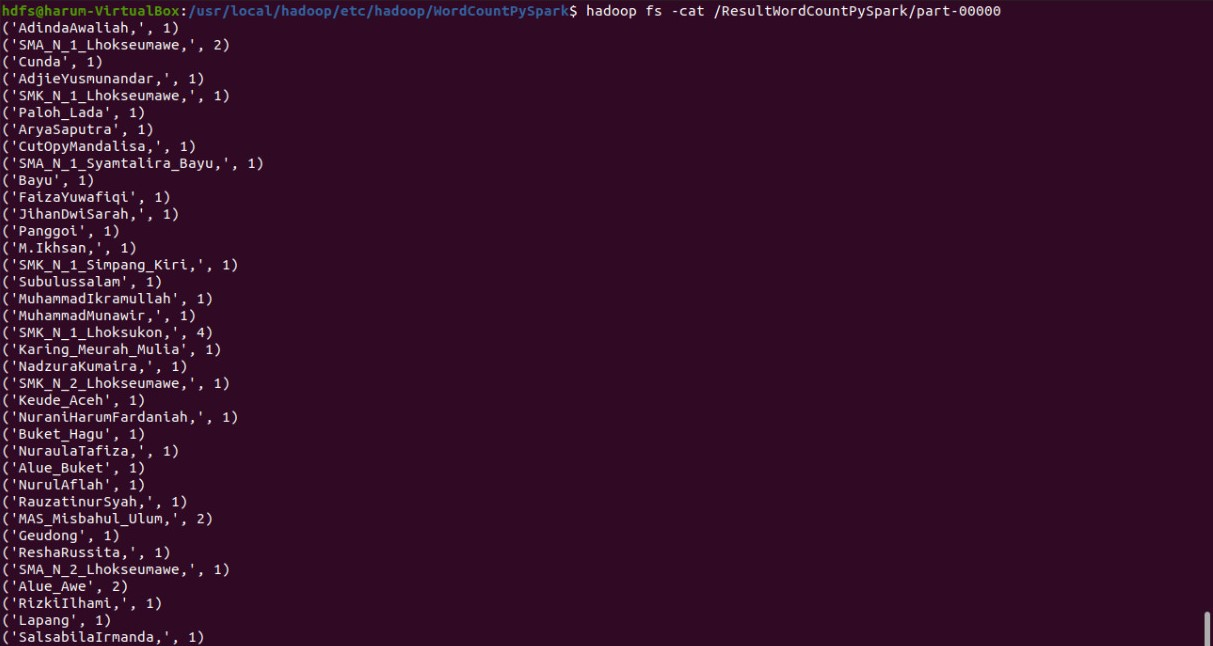
\includegraphics[width=\textwidth]{NuraniHarumFardaniah/pyspark7a}
\caption{Lihathasil ResultWordCountPyspark}
\label{gam:perkuliahan-25-11}
\end{figure}

\begin{figure}[!ht]
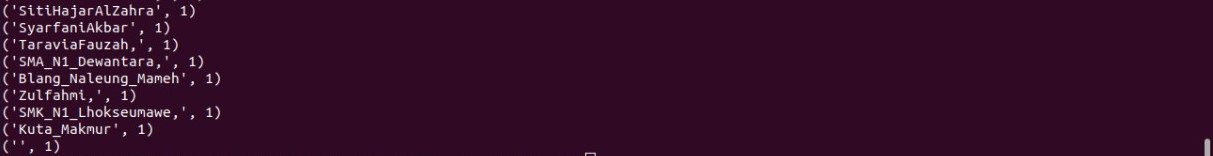
\includegraphics[width=\textwidth]{NuraniHarumFardaniah/pyspark7b}
\caption{Lihat hasil ResultWordCountPyspark}
\label{gam:perkuliahan-25-11}
\end{figure}
\end{enumerate}
